\documentclass{article}

\usepackage[top=1in, bottom=1.25in, left=1.25in, right=1.25in]{geometry}
\usepackage[utf8]{inputenc}
\usepackage[english]{babel}

\usepackage{amsmath}
\usepackage{amssymb}

\usepackage[numbers]{natbib}
\usepackage[colorlinks=true, linkcolor=blue, citecolor=blue, urlcolor=blue]{hyperref}
% \usepackage{listings}
% \lstset{
%   basicstyle=\textbf\normalsize\ttfamily,
%   }
\newcommand{\code}[1]{\textbf{\normalsize\ttfamily #1}}

% \usepackage{wasysym}
\usepackage{graphicx}
\usepackage{siunitx}

\title{Notes on a numerical solver for the Hartree-Fock equation of state of a homogeneous Bose gas}
\author{Carmelo Mordini}

\begin{document}
\maketitle

\subsection*{Intro}

As reported in Giorgini's notes \cite{giorgini}, the thermodymanics of an homogenous gas of interacting bosons can be obtained analytically in a mean field approximation from the hamiltonian

\begin{equation}
  H_{HF} - \mu N = -gnN - \frac{g n_0 N_0}{2} + \sum_{k} \left(\epsilon_k - \mu + 2gn\right)a^\dagger_k a_k
\end{equation}
The equation of state is

~\\


% first column
\begin{minipage}[t]{0.5\textwidth}
\centering
Non-condensed phase
\begin{equation}
  \left\{
  \begin{aligned}
    n &= \frac{1}{\lambda_T^3}\, g_{3/2}(e^{\beta(\mu - 2gn)}) \\
    p &= g n^2 + \frac{k_B T}{\lambda_T^3}\, g_{5/2}(e^{\beta(\mu - 2gn)})
  \end{aligned}\right.
\end{equation}

\end{minipage}%
%second column
\begin{minipage}[t]{0.5\textwidth}
\centering
Condensed phase
\begin{equation}
  \left\{
  \begin{aligned}
    n &= n_0 + \frac{1}{\lambda_T^3}\, g_{3/2}(e^{\beta(\mu - 2gn)}) \\
    \mu &= 2gn - gn_0 \\
    p &= g n^2 -\frac{1}{2}gn_0^2 + \frac{k_B T}{\lambda_T^3}\, g_{5/2}(e^{\beta(\mu - 2gn)})
  \end{aligned}\right.
\end{equation}
\end{minipage}

\subsection*{Numerical solver}
We're looking for a tool \cite{hfsolver} that solves the equations and gives us the density and the condensed fraction as a function of $\mu$ and $T$, which are the parameters driving the equations above. So given $\mu$ and $T$ and of course the atomic quantities ($m$, $g$, $\hbar$ etc.) we rewrite everything in the rescaled units
\begin{equation}
\left\{
\begin{aligned}
  x = n \lambda_T^3 &\quad  x_0 = n_0 \lambda_T^3  &\text{density}\\
  \alpha &= \beta\frac{g}{\lambda_T^3}  &\text{temperature parameter}\\
  \nu &= \mu \frac{\lambda_T^3}{g} &\text{chemical potential}
\end{aligned}\right.
\end{equation}

And the equations for the density will read
~\\

% first column
\begin{minipage}[t]{0.5\textwidth}
\centering
Non-condensed phase
\begin{equation}\label{eq:non_cond}
    x = g_{3/2}(e^{\alpha(\nu - 2x)})
\end{equation}

\end{minipage}%
%second column
\begin{minipage}[t]{0.5\textwidth}
\centering
Condensed phase
\begin{equation}\label{eq:cond}
  \left\{
  \begin{aligned}
    x &= x_0 + g_{3/2}(e^{\alpha(\nu - 2x)}) \\
    \nu &= 2x - x_0 \\
  \end{aligned}\right.
\end{equation}
\end{minipage}

Let's find a solution for them.

\subsubsection*{Non-condensed phase}
Eq.~\ref{eq:non_cond} defines implicitly the density of the gas in the case where the condensed fraction is 0. It's useful to change variable to $z = e^{\alpha(\nu - 2x)}$, which is the fugacity, substitute for it and numerically find the zero of the function
\begin{equation}
  F(z; \alpha, \nu) = g_{3/2}(z) - \frac{\nu}{2} + \frac{1}{2\alpha}\ln z
\end{equation}
within the domain $z \in [0, 1]$.

Given that $F$ is monotonically increasing in $z$ and $F(0) = -\infty$, there exists a unique solution \textit{if and only if} $F(1) = g_{3/2}(1) - \frac{\nu}{2} \geq 0$, that is
\begin{equation}
  \nu \leq 2\,g_{3/2}(1) \simeq 5.224
\end{equation}
Figure~\ref{fig:solve_noncond} shows an example of solution, plotting $g_{3/2}(z)$ and $x(z) = \frac{\nu}{2} - \frac{1}{2\alpha}\ln z$ for a fixed value of temperature ($\alpha$), and for different $\nu$.
\begin{figure}
  \centering
  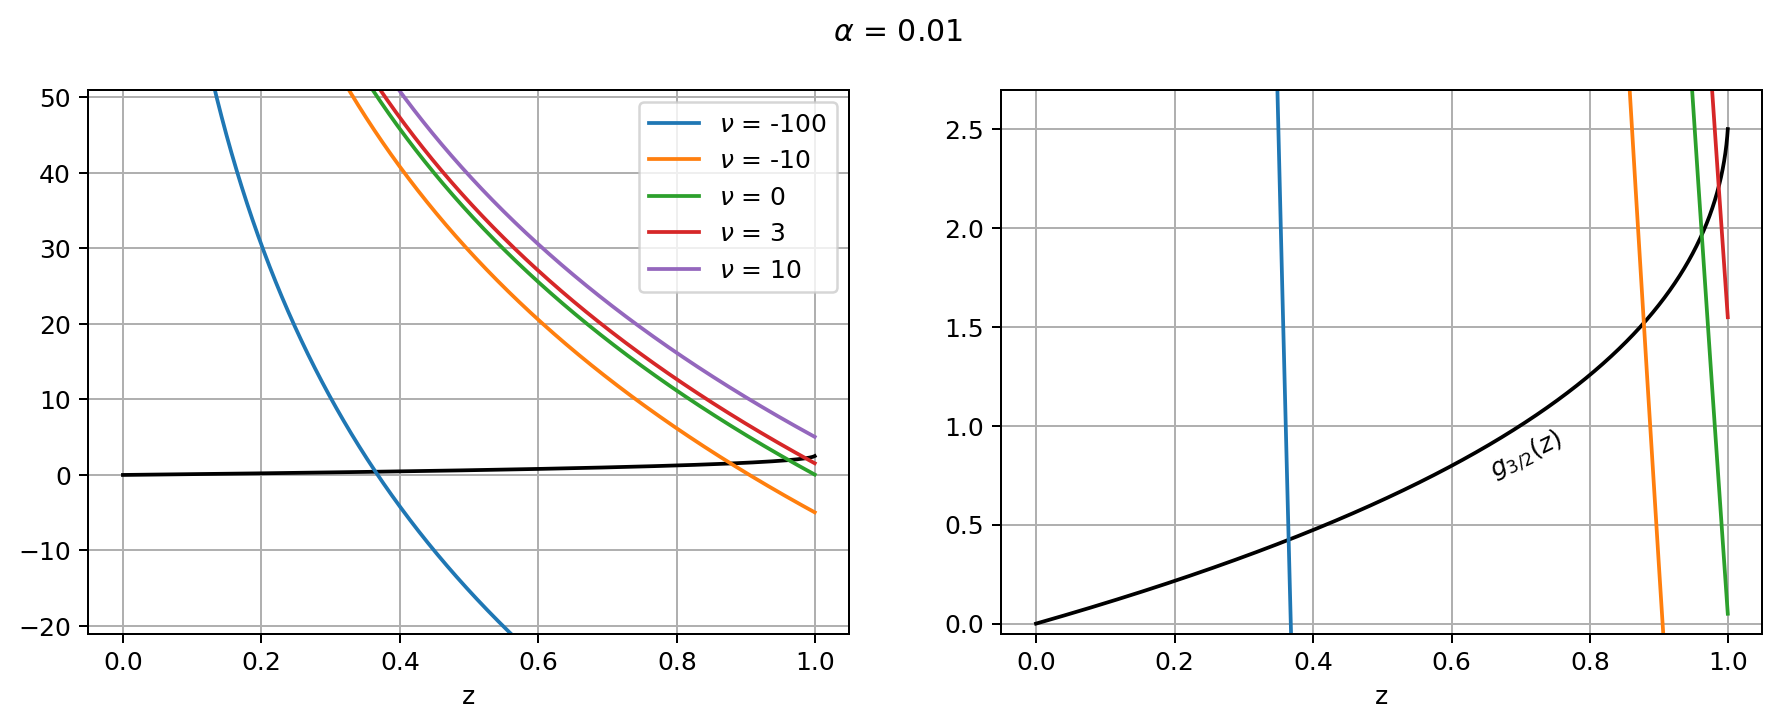
\includegraphics[width=0.8\textwidth]{figures/fig_solve_noncond}
  \caption{Root finding in the non-condensed phase}
  \label{fig:solve_noncond}
\end{figure}
In this phase the total density coincides with the thermal fraction, so from the fugacity we can calculate the non-condensed and condensed densities as
\begin{equation}
  \left\{
  \begin{aligned}
    x_t &= \frac{\nu}{2} - \frac{1}{2\alpha}\ln z \\
    x_0 &= 0
  \end{aligned}
  \right.
\end{equation}
Limited accuracy will affect the result when $z$ is close to its boundaries, that is for $z$ close to 1 (BEC threshold) or for $z$ close to 0 (deep thermal sample). In the latter case, corresponding to a large and negative $\nu$, both the fugacity and the density are expected to be small and one can carry out the following approximations:
\begin{align*}
  &\nu - 2x \simeq \nu \\
  &g_{3/2}(z) \simeq z
\end{align*}
resulting in the exponential density of a non interacting classical gas
\begin{equation}
  x_t = e^{\alpha \nu}
\end{equation}
Empirically, this is accurate (within machine precision) well before the numerical solution starts being unstable due to numerical errors, that is for $\nu \leq -10^3$.

\subsubsection*{Condensed phase}
\begin{figure}
  \centering
  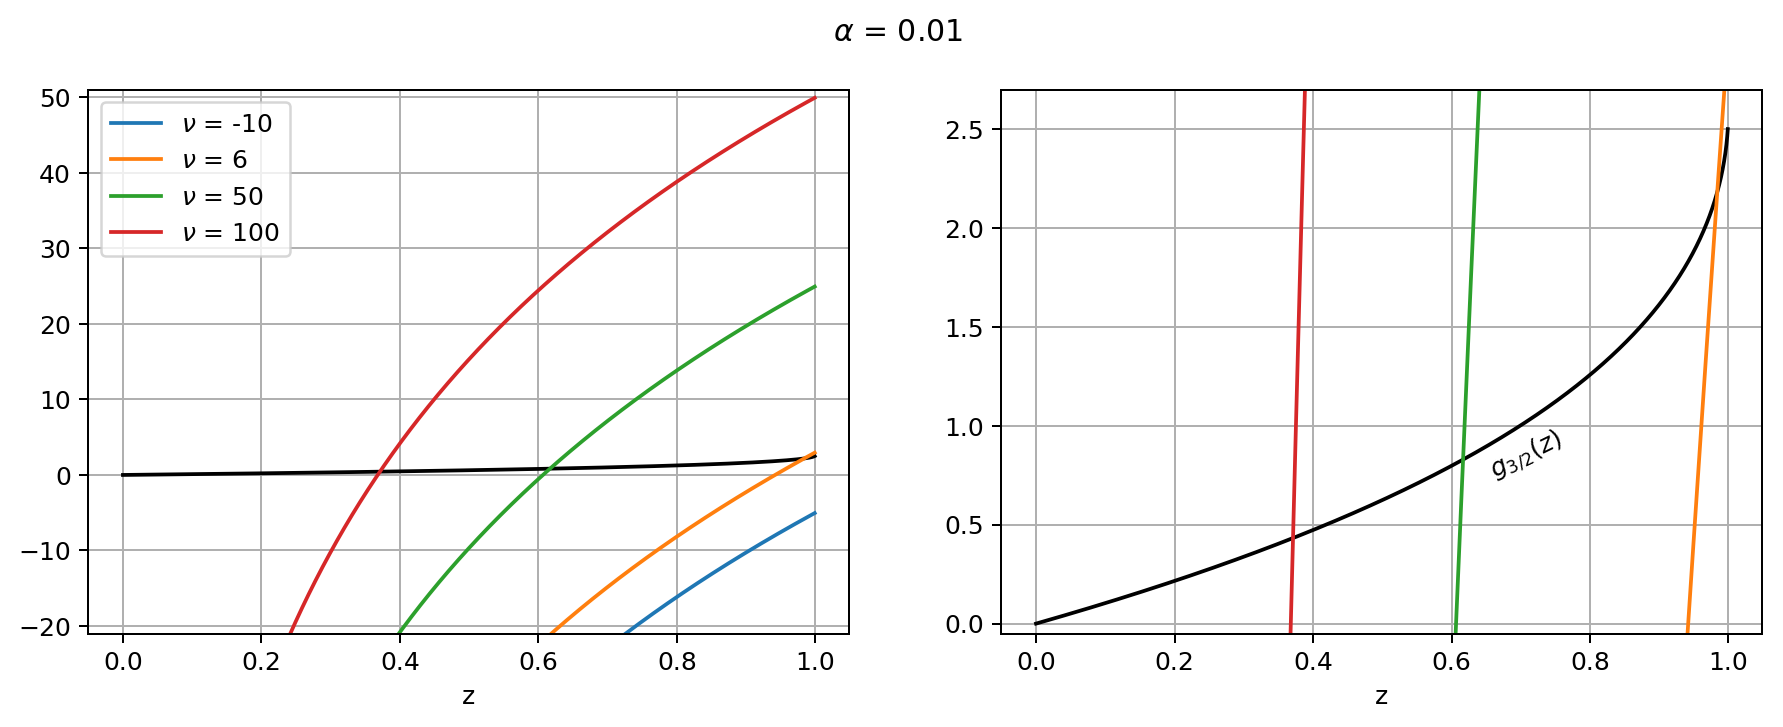
\includegraphics[width=0.8\textwidth]{figures/fig_solve_cond}
  \caption{Root finding in the condensed phase}
  \label{fig:solve_cond}
\end{figure}
We use the second of Eq.~\ref{eq:cond} to eliminate $x_0$ and make the same substitution for $x$ as a function of the fugacity $z$, obtaining the function
\begin{equation}
  F(z; \alpha, \nu) = g_{3/2}(z) - \frac{\nu}{2} - \frac{1}{2\alpha}\ln z
\end{equation}
which is almost the same as the previous one, except for a sign change. Now a unique solution always exists provided that $\nu \geq 2 g_{3/2}(1)$, which is the correct range of parameters where to use this functional form. An example plot is shown in Fig.~\ref{fig:solve_cond}. Beware that trying to solve this equation in the wrong range can lead to no solution or to two solutions, depending on the value of $\alpha$, but neither of the two is physically correct.\\
Calculating the total density $x$ from the solution for $z$ and substituting back in Eq.~\ref{eq:cond} we get the results for the thermal and condensed densities:
\begin{equation}
  \left\{
  \begin{aligned}
    x_t &= \frac{\nu}{2} + \frac{1}{2\alpha}\ln z \\
    x_0 &= \nu - 2 x_t
  \end{aligned}
  \right.
\end{equation}

\subsubsection*{Summary}
% Def. $\zeta = g_{3/2}(1)$,
\begin{equation*}
  \left\{
  \begin{aligned}
    &(\nu \leq 2\,g_{3/2}(1)) \quad F(z) = g_{3/2}(z) - \frac{\nu}{2} + \frac{1}{2\alpha}\ln z \quad\Rightarrow\quad
      \left\{
      \begin{aligned}
      x_t &= \frac{\nu}{2} - \frac{1}{2\alpha}\ln z \\
      x_0 &= 0
      \end{aligned}\right. \\
    &(\nu > 2\,g_{3/2}(1)) \quad F(z) = g_{3/2}(z) - \frac{\nu}{2} - \frac{1}{2\alpha}\ln z \quad\Rightarrow\quad
      \left\{
      \begin{aligned}
        x_t &= \frac{\nu}{2} + \frac{1}{2\alpha}\ln z \\
        x_0 &= \nu - 2 x_t
      \end{aligned}\right.
  \end{aligned}
  \right.
\end{equation*}

Figure~\ref{fig:solution} shows a solution for $x_0$, $x_t$ close to the transition point.

\subsection*{A bit of physics}
\subsubsection*{Reasonable values}

Assuming a sample of Na$^{23}$ atoms, Fig.~\ref{fig:alpha_nu} shows a range of physically plausible values for $\alpha(T)$ and $\nu(\mu, T)$.

\subsubsection*{Harmonic trap}

The above equations can be used to predict the density distribution in a inhomogeneous system assuming Local Density Approximation (LDA): in an external potential $V(x)$ one can think each point as being a locally homogeneous sample, whose density is determined by a local chemical potential $\mu(x) = \mu_0 - V(x)$.

Fig.~\ref{fig:harmonic_trap} shows the radial density profile of a trapped BEC of Na$^{23}$ atoms, in a spherical harmonic potential with trap frequency $\omega = 2 \pi \times \SI{60}{Hz}$, at $T = \SI{300}{nK}$ and $\mu_0 = k_B\times\SI{130}{nK}$. The corresponding adimensional parameters are $\alpha \sim 0.0082$ and $\nu$ ranging from 50 in the center to -430 at a radius of \SI{80}{\micro m}. This results in a sample of $\sim 6\times 10^6$ atoms and a BEC fraction $N_0/N \sim 60\,\%$.


\begin{figure}
  \centering
  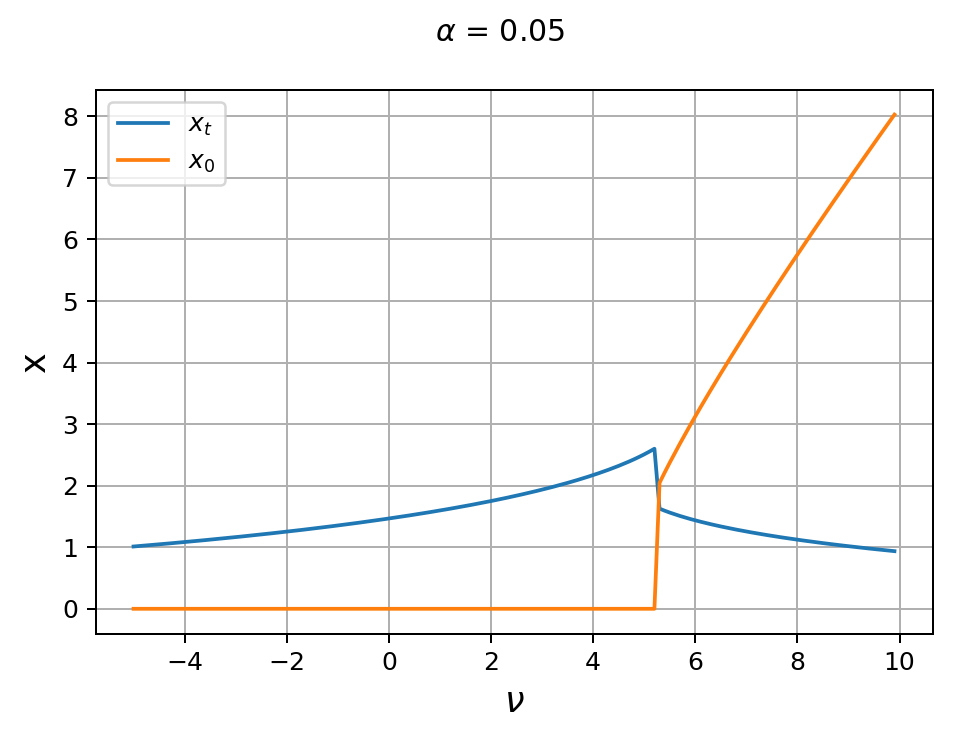
\includegraphics[width=0.6\textwidth]{figures/fig_n_mu}
  \caption{Example solution: thermal and condensed densities vs $\nu$}
  \label{fig:solution}
\end{figure}

\begin{figure}
  \centering
  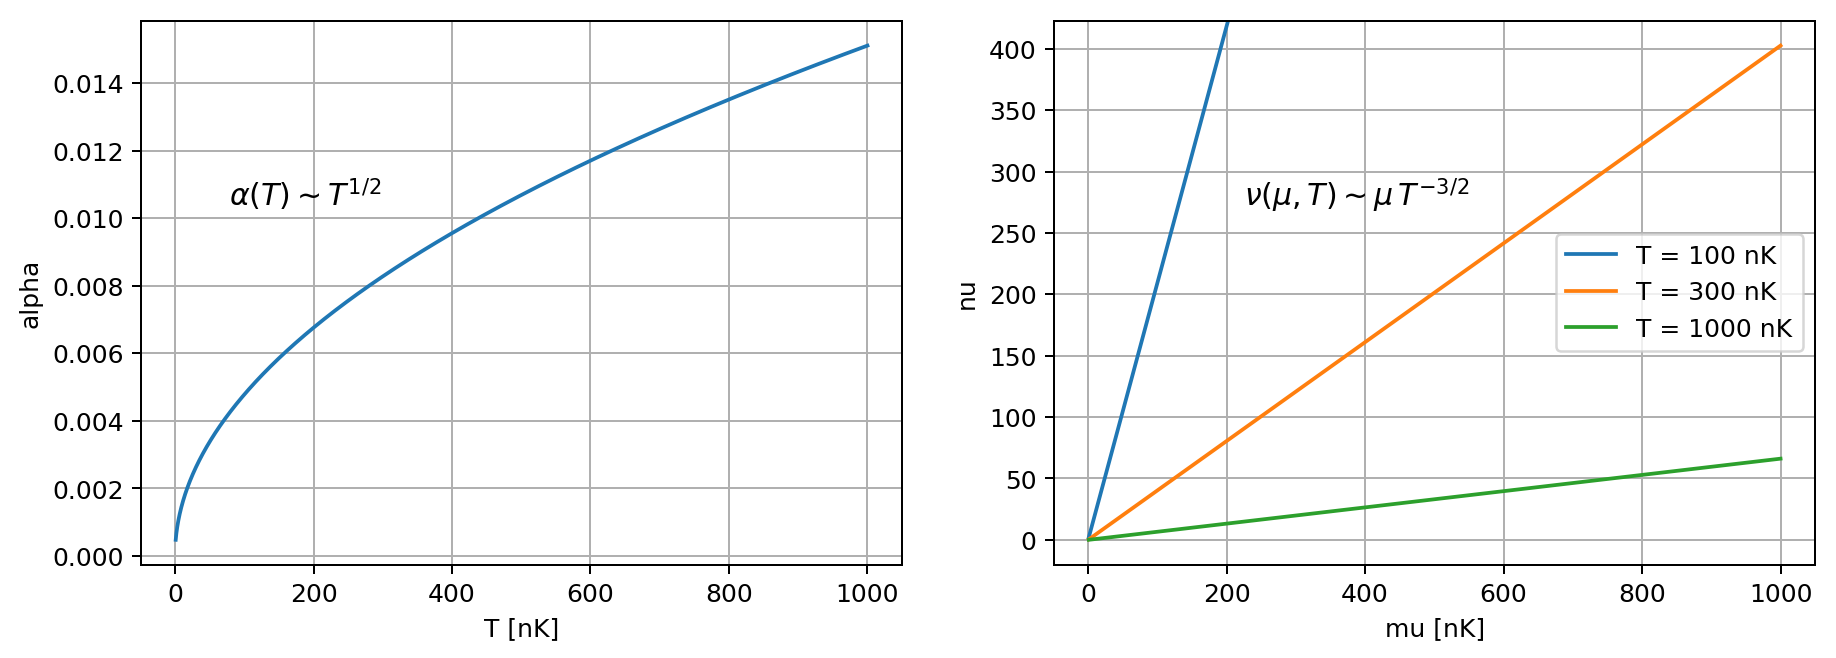
\includegraphics[width=\textwidth]{figures/fig_alpha_nu}
  \caption{Physical values for $\alpha(T)$, $\nu(\mu, T)$}
  \label{fig:alpha_nu}
\end{figure}

\begin{figure}
  \centering
  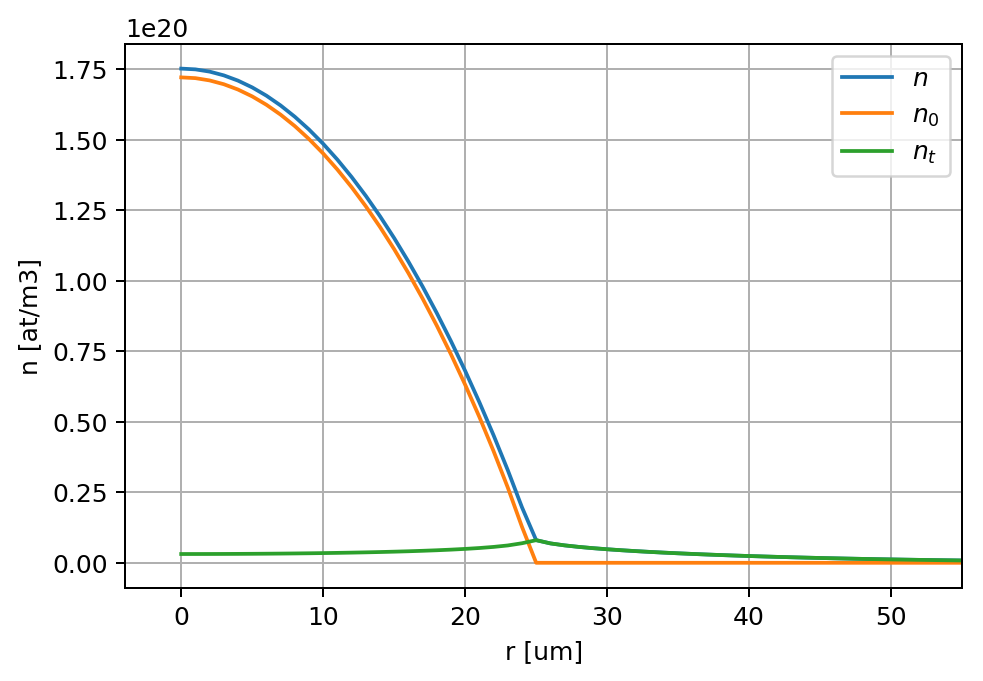
\includegraphics[width=\textwidth]{figures/fig_harmonic_trap}
  \caption{Density of a trapped condensate in a spherical harmonic potential}
  \label{fig:harmonic_trap}
\end{figure}

\begin{thebibliography}{}
\pagestyle{headings}
\bibitem{giorgini} non lo trovo su internet
\bibitem{hfsolver} \url{https://github.com/carmelom/hfsolver}
\end{thebibliography}


\end{document}
